\chapter{The Standard Model of Particle Physics}\label{ch:sm}

The Standard Model is a set of theories describing the interactions between elementary particles.
It explains three of the four known fundamental forces, namely the electromagnetic force,
the weak nuclear force, and the strong force.
It does not include  or account for gravitational interactions.

The Standard Model can be fairly characterized as one of the most successful theories in science.
A huge number of predictions made by the theory have been confirmed experimentally,
some to an astounding degree of accuracy.
Precision measurements of the magnetic moment of the electron have shown the experimental and theoretical values of the
fine structure constant to agree better than one part in one billion.\cite{sm-fine-structure-2008}
The ATLAS detector at the LHC has confirmed the predicted rate of particle production for a very wide range of
production processes and final states.
A summary of Standard Model measurements made by ATLAS, and their comparisons to theoretical predictions can be seen in figure~\ref{fig:sm_xsec_summary}.
The Standard Model predicted the existence of the W boson, the top quark, and the Higgs boson,
which were all later confirmed by experiment.

\begin{figure}[h!]
    \centering
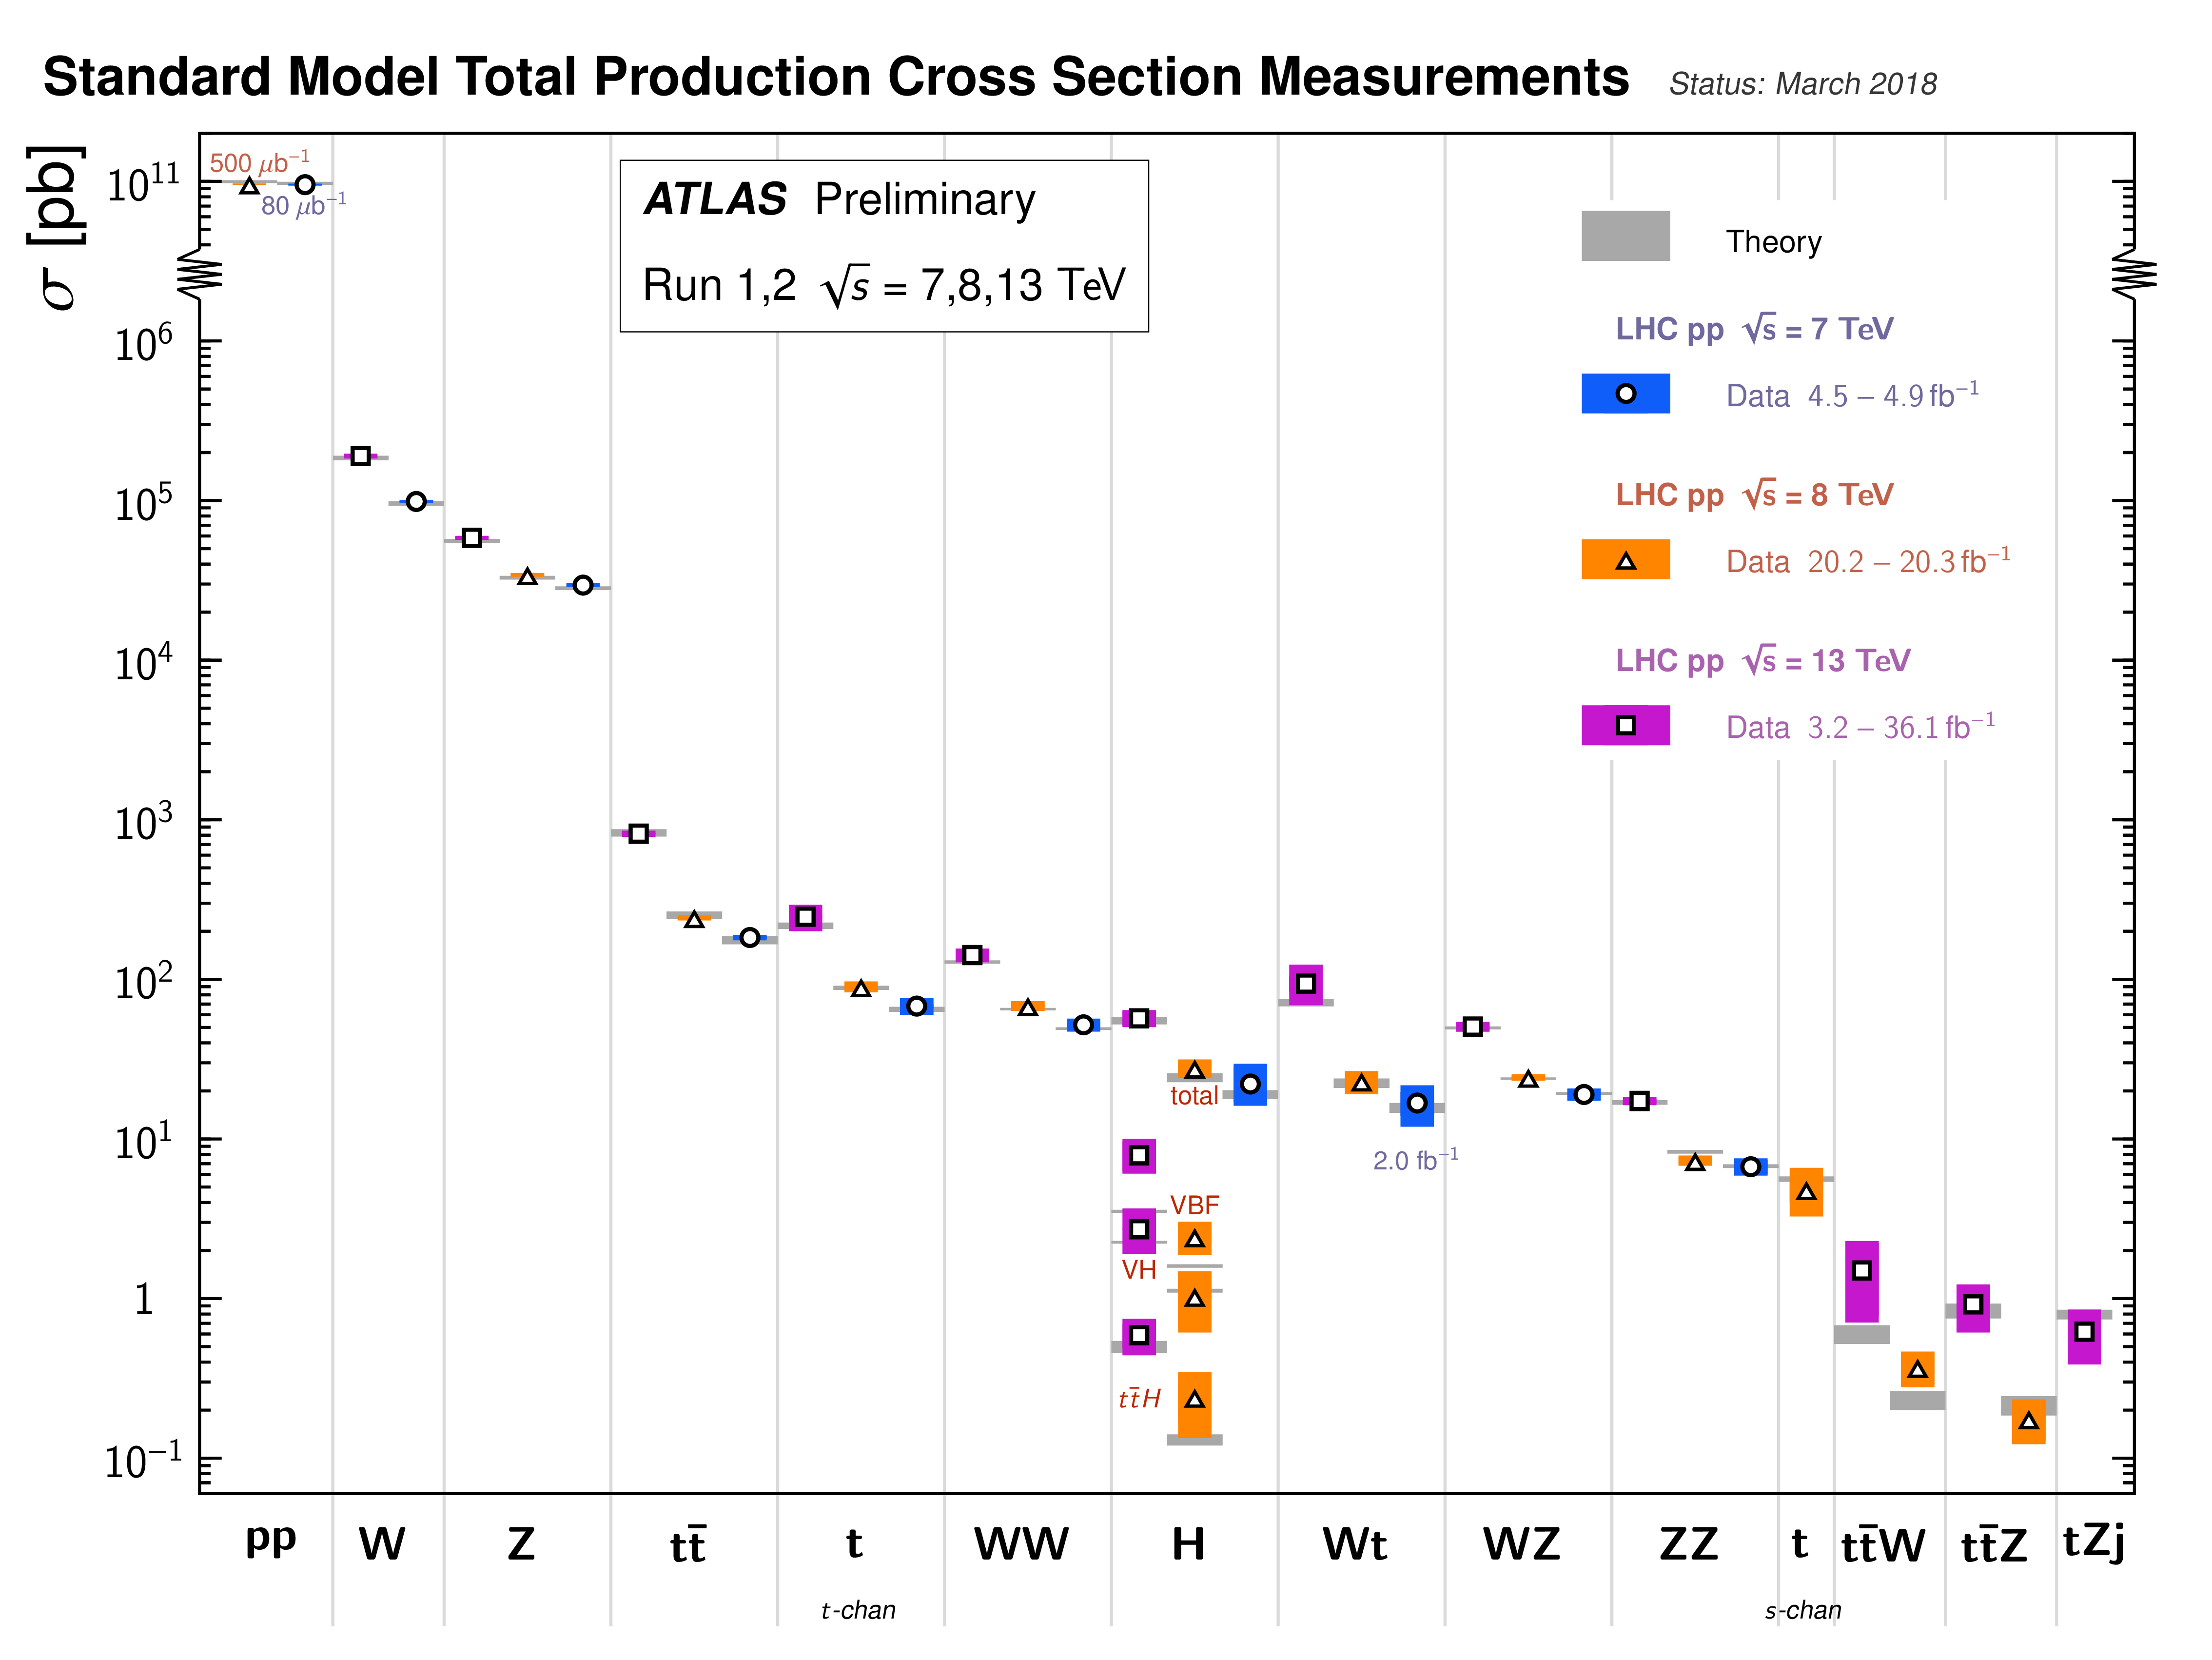
\includegraphics[width=0.6\linewidth]{sm_xsec_summary}
\caption{Summary of Standard Model production cross sections measured by ATLAS, compared to theoretical predictions.}
\label{fig:sm_xsec_summary}
\end{figure}

The Standard Model is expressed in the language of Quantum Field Theory.
The theory consists of three generations of matter fields,
specified by their representation under the gauge group $SU(3)\times SU(2)\times U(1)$ and the Poincar\'e group,
as well as a complex scalar field.
Poincar\'e symmetry consists of the Lorentz symmetry of special relativity, plus global translational symmetry.

The Standard Model is a complete theory in the sense that it is internally self-consistent,
and all particles predicted by the theory have been discovered experimentally.
However, the Standard Model does not account for all known physical phenomena,
and so cannot be considered a complete theory of nature.

\section{Electroweak Sector and the Higgs Mechanism}\label{sec:sm_ew}

\subsection{Matter fields}\label{subsec:ew_fields}

All left-handed matter fields are $SU(2)$ doublets, while their corresponding right-handed fields are $SU(2)$ singlets.
There are three generations of left-handed lepton fields:

\begin{equation}\label{eq:left_handed_leptons}
    \begin{pmatrix}
        \nu_e \\ l_e
    \end{pmatrix}_L,\;
    %
    \begin{pmatrix}
        \nu_{\mu} \\ l_{\mu}
    \end{pmatrix}_L,\;
    %
     \begin{pmatrix}
        \nu_{\tau} \\ l_{\tau}
    \end{pmatrix}_L
\end{equation}

And three generations of right-handed lepton fields:
\begin{equation}\label{eq:right_handed_leptons}
e_R,\; \mu_R,\; \tau_R
\end{equation}

Similarly, there are three generations each of the left-handed $SU(2)$-doublet quark fields,
each of which comes in three colors:

\begin{equation}\label{eq:left_handed_quarks}
    \begin{pmatrix}
        q_u \\ q_d
    \end{pmatrix}_L,\;
    %
    \begin{pmatrix}
        q_{c} \\ q_{s}
    \end{pmatrix}_L,\;
    %
     \begin{pmatrix}
        q_{t} \\ q_{b}
    \end{pmatrix}_L
\end{equation}


Quark color will play a role in QCD interactions, as discussed in the next session.
There are also the corresponding $SU(2)$-singlet right-handed fields:

\begin{equation}\label{eq:right_handed_quarks}
q_{uR},\; q_{dR},\; q_{cR},\; q_{sR},\; q_{tR},\; q_{bR}
\end{equation}

\subsection{Symmetries and Lagrangian}\label{subsec:ew_lagrangian}
The symmetry constraining the electroweak sector of the Standard Model Lagrangian is $SU(2)_L \times U(1)_Y$.
The subscript $L$ for the $SU(2)$ group indicates that it only acts on the left-handed fields in the theory.
Right-handed fields appear as $SU(2)$ singlets.
The Lagrangian density satisfying the required symmetries, including all renormalizable terms, is:

\begin{equation}\label{eq:ew_lagrangian}
    \mathcal{L} = -\frac{1}{4}W^{\mu \nu}_{a}W_{\mu \nu}^{a}-\frac{1}{4}B^{\mu \nu}B_{\mu \nu}
\end{equation}

Where $W_\mu^a$ are the three $SU(2)_L$ gauge bosons, $B_\mu$ is the $U(1)_Y$ (hypercharge) gauge boson,
and $W_\mu\nu = \delta_{\mu} W_{\nu} - \delta_{\nu} W_{\mu}$.

This Lagrangian describes the charged-current and neutral-current interactions, as well as gauge-boson self-interactions.
However, it is insufficient because the gauge bosons are massless.
In fact, it is impossible to include gauge boson mass terms in the electroweak Lagrangian without explicity breaking the gauge symmetry.

\subsection{Higgs mechanism}\label{subsec:ew_higgs}

The original symmetry is spontaneously broken, via the nonzero Higgs vacuum expectation value, to: $U(1)_{QED}$.
This process of spontaneous symmetry breaking generates fermion masses, electroweak gauge boson masses, and the Yukawa coupling terms between fermions.

\section{Quantum Chromodynamics}\label{sec:sm_qcd}

\section{Phenomenology}\label{sec:sm_pheno}

\section{Limitations}\label{sec:sm_limits}
